\chapter{Конечные автоматы}
\label{Chapter3}

\section{Определения и примеры}
\label{Chapter3Defines}

\mydef{Конечный автомат} является одним из простейших
распознавателей (см.~\ref{Chapter1Parsers}). Он состоит из входной ленты и
управляющего устройства с конечной памятью. Управляющее
устройство может быть недетерминированным. Входную
головку далее будем полагать односторонней, более того,
фактически мы потребуем, чтобы входная головка сдвигалась
вправо на каждом такте.

\mydef{Недетерминированным конечным} автоматом называется пятерка
\[
    M = (Q,\Sigma, \delta, q_0, F),
\]
где $Q$ --- конечное множество состояний, $\Sigma$ --- конечное
множество допустимых входных символов, $\delta$ --- отображение
множества $\Sigma$ во множество $P(Q)$ всех подмножеств множества $Q$,
$q_0$ ($\in Q)$ --- начальное состояние управляющего устройства,
$F$ ($\subseteq Q)$ --- множество заключительных состояний.

Функцию $\delta$ называют \mydef{функцией переходов}, именно она
фактически определяет поведение управляющего устройства. Функция
переходов по данному <<текущему>> состоянию и <<текущему>> входному
символу указывает набор всех возможных следующих состояний. Нестрого
говоря, автомат дублирует себя так, что в каждом из возможных следующих
состояний находится как бы один из равноправных экземпляров этого
устройства; при этом недетерминированный автомат допускает входное
слово в том случае, если какой"/нибудь из его параллельно работающих
экземпляров достигает допускающего состояния.

<<Недетерминизм>> конечного автомата не следует смешивать со
<<случайностью>>, при которой автомат может случайно выбрать одно из
следующих состояний с фиксированными вероятностями, но этот автомат
всегда имеется только в одном экземпляре. Такой автомат называется
<<вероятностным>>, и мы его изучать не будем.

Детерминированный конечный автомат определим как частный случай
недетерминированного. Именно, пусть $M = (Q,\Sigma,
\delta, q_0, F)$ --- недетерминированный конечный автомат. Автомат $M$
назовем \mydef{детерминированным}, если множество $\delta(q,a)$
содержит не
более одного состояния для любых $q\in Q$ и $a\in\Sigma$. Если
$\delta(q,a)$ содержит точно одно состояние, то автомат $M$ назовем
\mydef{полностью определенным}.

Работа конечного автомата представляет собой некоторую последовательность тактов. Такт определяется текущим состоянием управляющего устройства и входным символом, считываемым в данный момент входной головкой. Сам такт состоит из изменения состояния и сдвига входной головки на одну ячейку вправо. Для того чтобы определить будущее поведение конечного автомата, нужно знать лишь текущее состоятие управляющего устройства и слово на входной ленте, состоящее из буквы под головкой и всех букв, расположенных вправо от неё. Эги два элемента информации дают мгновенное описание конечного автомата, которое называют конфигурацией. Другими словами, если $M = (Q,\\ \Sigma, \delta, q_0, F)$ --- конечный автомат, то пара $(q,\omega)\in Q*\Sigma^*$ называется конфигурацией автомата $M$. Конфигурация $(q_0\omega)$ называется начальной, а конфигурация $(q,\eps)$, где $q\in F$, называется заключительной.

Состояние $p$ называется достижимым, если существует такое слово $\omega$, что $(q_0,\omega)\vdash^*(p,\eps)$.

Такт автомата $M$ представляется бинарным отношением $\vdash_M$ (или, короче, $\vdash$), определенным на конфигурациях: если $q'\in\delta(q,a)$, то $(q,a\omega)\vdash(q',\omega)$ для всех $\omega\in\Sigma^*$. Таким образом, если $M$ находится в состоянии $q$ и входная головка обозревает входной символ $a$, то автомат $M$ может делать такт, за который он переходит в состояние $q'$ сдвигает головку на одну ячейку вправо. Так как автомат $M$, вообще говоря, может быть недетерминированным, то могут быть и другие состояния, в которые он тоже может перейти за один такт.

Запись $C\vdash_M^0 C'$ означает, что $C=C'$, а $C_0\vdash_M^kC_k$ для $k\ge 1$ --- что существуют такие конфигурации $C_i, \ldots ,C_{k-1}$, что $C_i\vdash_MC_{i+1}$ $0\le i<k$. Запись $C\vdash_M^+C'$ означает, что $C\vdash_M^kC'$ для некоторого $k\ge 1$, а $C\vdash_M^*C'$ --- что $C\vdash_M^k$ для некоторого $k\ge 0$. Будем опускать нижний индекс $M$ там, где это не приведет к недоразумениям.

Говорят, что автомат $M$ допускает слово $\omega$, если $(q_0,\omega)\vdash^*(q,\eps)$ для некоторого $q\in F$. Языком, допускаемым (определяемым, распознаваемым) автоматом $M$, называется множество $L(M)$ всех входных слов, допускаемых автоматом $M$, т. е.
\[
	L(M)=\{\omega(\in\Sigma^*)\mid~\exists q\in F\colon (q_0,\omega)\vdash^*(q,\eps)\}.
\]

Рассмотрим два конечных автомата, один из которых является детерминированным (пример~\ref{example-chap3-DKA1}), а второй --- недетерминированным (пример~\ref{aut-312}).

\begin{myexample}
\label{example-chap3-DKA1}
Пусть $M=(\{p;q;r\},\{0;1\},\delta,p,\{r\})$ --- конечный автомат, где функция переходов $\delta$ задаётся таблицей с рисунка~\ref{tab1}.
Этот автомат допускает все слова из нулей и единиц, содержащие два стоящих рядом нуля. Начальное состояние $p$ можно интерпретировать так: <<два стоящих рядом нуля еще не появились, и предыдущая буква не нуль>>. Состояние $q$ означает, что <<два стоящих рядом нуля еще не появились, но предыдущая буква --- нуль>>. Состояние $r$ означает, что <<Два стоящих рядом нуля уже появились>>. Попав в состояние $r$, автомат остается в этом состоянии навсегда.

\begin{table}
\centering
\begin{tabular}{cccc}
\toprule
%
\multicolumn{2}{c}{\multirow{2}{*}{\Large $\delta$}}
	& \multicolumn{2}{c}{\text{Вход}} \\
%
\cmidrule(lr){3-4}
%
\multicolumn{2}{c}{}
	& 0  & 1                          \\
%
\midrule
%
\multirow{3}{*}{\text{Состояние}}%
    &  $p$ & $\{q\}$ & $\{p\}$		  \\
    &  $q$ & $\{r\}$ & $\{p\}$		  \\
    &  $r$ & $\{r\}$ & $\{r\}$		  \\
\bottomrule
\end{tabular}
\caption{Функция перехода $\delta$ для автомата из примера~\ref{example-chap3-DKA1}.}
\label{tab1}
\end{table}


Например, если на вход автомата поступило слово $\omega=1010011$, то единственно возможной последовательностью конфигураций, начинающейся с конфигурации $(p,1010011)$, будет следующая последовательность:
\begin{multline*}
(p,1010011)
    \vdash\\(p,010011)
    \vdash(q,10011)
    \vdash(p,0011)
    \vdash(q,011)
    \vdash(r,11)
    \vdash(r,1)
    \vdash\\(r,\eps).
\end{multline*}
Таким образом, $1010011\in L(M)$.
\end{myexample}

Далее в случае детерминированных конечных автоматов мы будем писать, как правило, $\delta(q,a)=p$ вместо $\delta(q,a)=\{p\}$. Если $\delta(q,a)=\es$, то мы часто будем говорить, что $\delta(q,a)$ не определено.

\begin{myproblem}
Построите конечный автомат $M=(Q,\Sigma,\delta,q_0,F)$, допускающий те и только те слова над алфавитом $\Sigma=\{0;1\}$, у которых встречается три стоящих рядом нуля, но после этого подслова нет двух стоящих рядом единиц.
\end{myproblem}

\begin{myproblem}
Покажите, что конечный автомат из примера~\ref{example-chap3-DKA1} допускает язык $(0+1)^*00(0+1)^*$.
\end{myproblem}

\begin{myexample}\label{aut-312}
Построим недетерминированный конечный автомат
\[M=(Q.\Sigma,\delta, q_0, F),
\]
допускающий те и только те слова над алфавитом $\Sigma=\{1;2;3\}$, у которых последняя буква уже появлялась раньше. Прежде всего введем так называемое нейтральное состояние $q_0$, в котором автомат не пытается ничего распознать. Введем также состояния $q_1$, $q_2$ и $q_3$, в каждом из которых $M$ делает предположение о том, что последняя буква слова совпадает с индексом состояния. Пусть $q_f$ --- одно заключительное состояние. Находясь в состоянии $q_0$, один из экземпляров автомата <<бездумно>> остаётся в нем и дальше, а другой экземпляр переходит в состояние $q_i$, если $i$ --- очередной символ. Находясь в состоянии $q_i$, один из экземпляров автомата, независимо от считываемой буквы, остаётся в нем и <<размышляет>> о том, что букву $i$ в слове он уже обнаружил, а именно она и может совпасть с последней буквой в слове. Другой же экземпляр, если видит букву $i$, сразу без всяких сомнений переходит в финальное состояние $q_f$. Из состояния $q_f$ автомат никуда не переходит, так как вопрос о том, допускается ли входное слово, решается только один раз, когда автомат сочтет входную букву последней. Итак, формально автомат определяется как пятерка
\[
	M=(\{q_0;q_1;q_2;q_3;q_f\},\{1;2;3\},\delta,q,\{q_f\}),
\]
где функция переходов $\delta$ задается таблицей с рисунка~\ref{tab2}.

\begin{figure}
\centering
\begin{tabular}{lllll}
\toprule
%
\multicolumn{2}{c}{\multirow{2}{*}{\Large $\delta$}}
	& \multicolumn{3}{c}{\text{Вход}} \\
%
\cmidrule(rl){3-5}
%
\multicolumn{2}{c}{}
	& \multicolumn{1}{c}{1}
    & \multicolumn{1}{c}{2}
    & \multicolumn{1}{c}{3} \\
%
\midrule
%
\multirow{5}{*}{Состояние}
    & $q_0$ & \{$q_0;q_1$\} & \{$q_0;q_2$\} & \{$q_0;q_3$\} \\
    %
    & $q_1$ & \{$q_1;q_f$\} & \{$q_1$\}     & \{$q_1$\}     \\
    %
    & $q_2$ & \{$q_2$\}     & \{$q_2;q_f$\} & \{$q_2$\}     \\
    %
    & $q_3$ & \{$q_3$\}     & \{$q_3$\}     & \{$q_3;q_f$\} \\
    %
    & $q_f$ & $\es$         & $\es$         & $\es$         \\
\bottomrule
\end{tabular}
\caption{Функция перехода $\delta$ для автомата из примера~\ref{aut-312}.}
\label{tab2}
\end{figure}


Работа этого автомата при чтении слова $\omega=12321$ проиллюстрирована схемой на рисунке~\ref{aut-312-sch}.

\begin{figure}
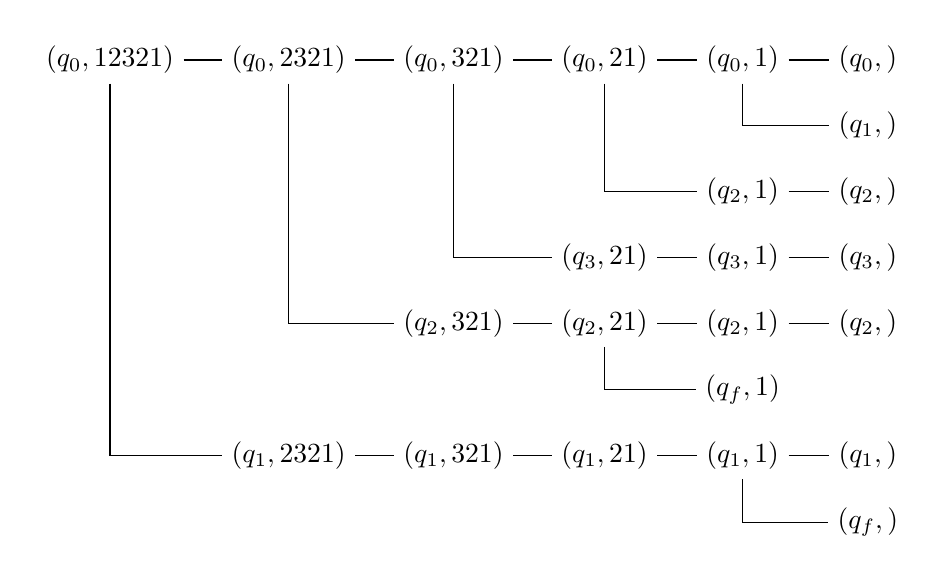
\begin{tikzpicture}
    \matrix (m1) [row sep=2.5mm, column sep=5mm]
    {
        \node (q012321) {$(q_0, 12321)$}; &
        \node (q02321)  {$(q_0, 2321)$};  &
        \node (q0321)   {$(q_0, 321)$};   &
        \node (q021)    {$(q_0, 21)$};    &
        \node (q01)     {$(q_0, 1)$};     &
        \node (q0eps)   {$(q_0, \eps)$};
        \\
        & & & & &
        \node (q1eps)   {$(q_1, \eps)$};
        \\
        & & & &
        \node (q21)     {$(q_2, 1)$};     &
        \node (q2eps)   {$(q_2, \eps)$};
        \\
        & & &
        \node (q321)    {$(q_3, 21)$};    &
        \node (q31)     {$(q_3, 1)$};     &
        \node (q3eps)   {$(q_3, \eps)$};
        \\
        & &
        \node (q2321)   {$(q_2, 321)$};   &
        \node (q221)    {$(q_2, 21)$};    &
        \node (q21X)    {$(q_2, 1)$};     &
        \node (q2epsX)  {$(q_2, \eps)$};
        \\
        & & & &
        \node (qf1)     {$(q_f, 1)$};     &
        \\
        &
        \node (q12321)  {$(q_1, 2321)$};  &
        \node (q1321)   {$(q_1, 321)$};   &
        \node (q121)    {$(q_1, 21)$};    &
        \node (q11)     {$(q_1, 1)$};     &
        \node (q1epsX)  {$(q_1, \eps)$};
        \\
        & & & & &
        \node (qfeps)     {$(q_f, \eps)$};
        \\
    };

    \draw (q012321)      -- (q02321) -- (q02321)
                          -- (q0321) -- (q021) -- (q01)  -- (q0eps);
    \draw (q01.south)    |- (q1eps);
    \draw (q021.south)   |- (q21)    -- (q2eps);
    \draw (q0321.south)  |- (q321)   -- (q31)  -- (q3eps);
    \draw (q02321.south) |- (q2321)  -- (q221) -- (q21X) -- (q2epsX);
    \draw (q221.south)   |- (qf1);
    \draw (q012321)      |- (q12321)
                          -- (q1321)  -- (q121) -- (q11)  -- (q1epsX);
    \draw (q11.south)    |- (qfeps);
\end{tikzpicture}
\caption{Схема работы автомата из примера~\ref{aut-312} на слове
$\omega=12321$.}
\label{aut-312-sch}
\end{figure}


Таким образом, возможна последовательность конфигураций:
\[
(q_0,12321)\vdash(q_1,2321)\vdash(q_1,321)\vdash(q_1,21)\vdash(q_1,1)\vdash(q_f,\eps).
\]
Это означает, что $12321\in L(M)$.
\end{myexample}

\begin{myproblem}
Докажите, что конечный автомат из примера~\ref{aut-312} допускает язык $\{\omega a\mid a\in\{1,2,3\}$ и $a$ входит в $\omega\}$. Постройте регулярное выражение для этого языка.
\end{myproblem}

\section[Редукция НКА к ДКА]{Редукция недетерминированных конечных автоматов к детерминированным}
\label{Chapter3Reduct}

В этом разделе будет доказано, что класс языков, определяемых недетерминизированными конечными автоматами, совпадает с классом языков, определяемых полностью определенными детерминизированными конечными автоматами. В силу этого произвольный язык из этого класса мы будем называть далее конечно"/автоматным.

\begin{mytheorem}
\label{theorem-reduction-NKAtoDKA}
Пусть $M=(Q,\Sigma,\delta,q_0,F)$ --- недетерминированный конечный автомат. Тогда существует такой детерминированый конечный автомат $M'$ что $L(M) = L(M')$.
\end{mytheorem}

\begin{myproof}
По данному недетерминированному автомату $M$ построим новый автомат $M=(Q',\Sigma,\delta ',q_0',F')$ следующим образом:
\begin{enumerate}
\item $Q'=P(Q)$, т.е. состояниями автомата $M'$ являются всевозможные подмножеста множества состояний автомата $M$;
\item Если $S\in Q'$, $a\in\Sigma$, то определим $\delta '(S,a)$ равенством
\[
	\delta '(S,a) = \bigcup_{q\in S} \{\delta(q,a)\};
\]

\item $q'_0=\{q_0\}$;

\item $F'$ состоит из всех таких подмножеств $S$ множества состояний $Q$, что \[
	S\cap F\neq\es.
\]
\end{enumerate}
Применяя метод математической индукции по $i$, нетрудно проверить, что $(S,\omega)\vdash_{M'}^i(S',\eps)$ в том и только в том случае, когда
\[
S'=\{p\mid\exists q\in S\colon (q,\omega)\vdash_M^i(p,\eps)\}
\]
Отсюда, в частности, следует, что $(\{q_0\},\omega)\vdash_{M'}^i(S',\eps)$ для некоторого $S'\in F'$ тогда и только тогда, когда $(q_0,\omega)\vdash_M^i(p,\eps)$ для некоторого $p\in F$. Итак, $L(M')=L(M)$.
\end{myproof}

\begin{myexample}
\label{example-NKAtoDKA-321}\label{aut-313}
Пусть
\[
M=(\{q_0;q_1;q_2;q_3;q_f\},\{1;2;3\},\delta,q,\{q_f\})
\]
недетерминированный конечный автомат, определенный в примере~\ref{aut-312}. Воспользуемся конструкцией из доказательства теоремы~\ref{theorem-reduction-NKAtoDKA} и построим полностью определенный детерминированный конечный автомат $M'=(Q',\{1;2;3\},\delta',\{q_0\},F')$, допускающий язык $L(M)$.

Так как автомат $M$ имеет пять состояний, то новый автомат $M'$ может иметь $32~(=2^5)$ состояния, однако не все они достижимы из начального. (Напомним, что состояние $p$ называется достижимым, если существует такое слово $\omega$, что $(q_0,\omega)\vdash^*(p,\eps)$.) Мы будем строить, естественно, только достижимые состояния.

Сделаем несколько полезных наблюдений.
\begin{enumerate}
    \item Очевидно, что состояние $\{q_0\}$ достижимо.

    \item Достижимыми являются состояния $\{q_0;q_a\}$ для
    $a\in \{1;2;3\}$; действительно,
    \[
        \delta'(\{q_0\}a)=\{q_0;q_a\}.
    \]

    \item Достижимыми являются состояния $\{q_0;q_a;q_f\}$ для $a\in\{1;2;3\}$; действительно, $\delta'(\{q_0;q_a\},a)=\{q_0;q_a;q_f\}$. Аналогично проверяется, что состояния $\{q_0;q_1;q_2\}$, $\{q_0;q_1;q_3\}$, $\{q_0;q_2;q_3\}$ --- достижимы.

    \item Из предыдущего факта легко выводится достижимость состояний
    \[
        \{q_0;q_1;q_2;q_3\}, \quad \{q_0;q_1;q_2;q_f\}, \quad
        \{q_0;q_1;q_3;q_f\}, \quad \{q_0;q_2;q_3;q_f\},
    \]
    а отсюда --- достижимость состояния $\{q_0;q_1;q_2;q_3;q_f\}$.
\end{enumerate}

Всего мы выявили 16 достижимых состояний. Анализ показывает, что подмножество $D$ множества состояний автомата $M$, т.е. состояние автомата $M'$, достижимо тогда и только тогда, когда выполняется условия: 1) $D$ содержит $q_0$, 2) если $D$ содержит $q_f$, то оно содержит также и $q_1$, $q_2$ или $q_3$. Легко видеть, что состояния, отличные от выделенных, не достижимы.

Итак, $Q'$ --- множество всех достижимых состояний автомата $M'$ --- состоит из 15 элементов и вместе с функцией переходов $\delta'$ представлено в таблице с рисунка~\ref{tab3} (с.~~\pageref{tab3}), где для простоты вместо состояний вида $\{q_i;q_j;\ldots ;q_k\}$ помещены списки $(i;j;\ldots ;k)$.

\begin{table}[H]
\centering
\begin{tabular}{llll}
\toprule
\multicolumn{1}{c}{\multirow{2}{*}{\Large $\delta^\prime$}}
	& \multicolumn{3}{c}{Вход} \\
\cmidrule(rl){2-4}
	& \multicolumn{1}{c}{1}
    & \multicolumn{1}{c}{2}
    & \multicolumn{1}{c}{3} \\
\midrule
$\{0\}$         & $\{0;1\}$       & $\{0;2\}$       & $\{0;3\}$       \\
$\{0;1\}$       & $\{0;1;f\}$     & $\{0;1;2\}$     & $\{0;1;3\}$     \\
$\{0;2\}$       & $\{0;1;2\}$     & $\{0;2;f\}$     & $\{0;2;3\}$     \\
$\{0;3\}$       & $\{0;1;3\}$     & $\{0;2;3\}$     & $\{0;3;f\}$     \\
$\{0;1;2\}$     & $\{0;1;2;f\}$   & $\{0;1;2;f\}$   & $\{0;1;2;3\}$   \\
$\{0;1;3\}$     & $\{0;1;3;f\}$   & $\{0;1;2;3\}$   & $\{0;1;3;f\}$   \\
$\{0;1;f\}$     & $\{0;1;f\}$     & $\{0;1;2\}$     & $\{0;1;3\}$     \\
$\{0;2;3\}$     & $\{0;1;2;3\}$   & $\{0;2;3;f\}$   & $\{0;2;3;f\}$   \\
$\{0;2;f\}$     & $\{0;1;2\}$     & $\{0;2;f\}$     & $\{0;2;3\}$     \\
$\{0;3;f\}$     & $\{0;1;3\}$     & $\{0;2;3\}$     & $\{0;3;f\}$     \\
$\{0;1;2;f\}$   & $\{0;1;2;f\}$   & $\{0;1;2;f\}$   & $\{0;1;2;3\}$   \\
$\{0;1;3;f\}$   & $\{0;1;3;f\}$   & $\{0;1;2;3\}$   & $\{0;1;3;f\}$   \\
$\{0;2;3;f\}$   & $\{0;1;2;3\}$   & $\{0;2;3;f\}$   & $\{0;2;3;f\}$   \\
$\{0;1;2;3\}$   & $\{0;1;2;3;f\}$ & $\{0;1;2;3;f\}$ & $\{0;1;2;3;f\}$ \\
$\{0;1;2;3;f\}$ & $\{0;1;2;3;f\}$ & $\{0;1;2;3;f\}$ & $\{0;1;2;3;f\}$ \\ \bottomrule
\end{tabular}
\caption{Функция перехода $\delta'$ для автомата из примера~\ref{aut-313}}\label{tab3}
\end{table}


Начальным состоянием автомата $M'$ является $\{q_0\}\in Q'$, а множество заключительных состояний $F'$ имеет вид:
\[\begin{array}{rllll}
F' = \{
	& \{q_0,q_1,q_f\};     & \{q_0,q_2,q_f\};     & \{q_0,q_3,q_f\};&\\
	& \{q_0,q_1,q_2,q_f\}; & \{q_0,q_1,q_3,q_f\}; & \{q_0,q_2,q_3,q_f\};&\\
	& & & \{q_0,q_1,q_2,q_3,q_f \} & \}.
\end{array}\]
\end{myexample}

\section{Граф переходов}
\label{Chapter3Graph}
Пусть $M=(Q,\Sigma,\delta,q_0,F)$ --- недетерминированный конечный автомат. Графом переходов (или диаграммой) автомата $M$ называют неупорядоченый помеченный граф, вершины которого помечены именами состояний; в графе есть дуга $(p,q)$, если существует такая буква $a\in\Sigma$, что $q\in\delta(p,a)$; кроме того, дуга $(p,q)$ помечается списком, состоящим из всех таких $a$, что $q\in\delta(p,a)$.

При изображении графа переходов условимся начальное состояние указывать направленной в него стрелкой, помеченной словом начало, а заключительные состояния обводить двойным кружком.

\begin{myexample}
Рассмотрим детерминированный конечный автомат из примера~\ref{example-chap3-DKA1}. Его граф переходов изображен на рисунке~\ref{aut-graph-1}.
\begin{figure}[H]
\centering
\begin{tikzpicture}[node distance=3cm,>=stealth',auto,every state/.style={thick}]
	\node (init) {};
	\node[state] (p) [right=.7cm of init] {$P$};
	\node[state] (q) [right of=p] {$q$};
	\node[state,accepting] (r) [right of=q] {$r$};

	\path[->]
    	(init) edge (p)
		(p) edge [loop above] node {$1$} (p)
		(p) edge node {$0$} (q)
		(q) edge [bend right] node[above] {$1$} (p)
		(q) edge node {$0$} (r)
        (r) edge [loop above] node {$0, 1$} (r);
\end{tikzpicture}
\caption{Граф переходов автомата из примера~\ref{example-chap3-DKA1}}
\label{aut-graph-1}
\end{figure}
\end{myexample}

\begin{myexample}
Рассмотрим недетерминированный конечный автомат из примера~\ref{aut-312}. Его граф переходов изображен на рисунке~\ref{aut-graph-2}.
\end{myexample}

\begin{figure}
\centering
\begin{tikzpicture}[auto,>=stealth', node distance=4cm,auto,every state/.style={thick}]
	\node (init) {};
	\node[state] (q0) [right=.7cm of init] {$q_0$};
	\node[state] (q1) [above right of=q0] {$q_1$};
    \node[state] (q2) [right of=q0] {$q_2$};
    \node[state] (q3) [below right of=q0] {$q_3$};
	\node[state,accepting] (qf) [right of=q2, above right of=q3] {$q_f$};

	\path[->]
    	(init) edge (q0)
		(q0) edge [loop above] node {$1, 2, 3$} (q0)
		(q0) edge node {$1$} (q1)
        (q0) edge node {$2$} (q2)
        (q0) edge node {$3$} (q3)
        (q1) edge [loop above] node[right] {$1, 2, 3$} (q1)
        (q1) edge node {$1$} (qf)
        (q2) edge [loop above] node[right] {$1, 2, 3$} (q2)
        (q2) edge node {$2$} (qf)
        (q3) edge [loop above] node[right] {$1, 2, 3$} (q3)
        (q3) edge node {$3$} (qf);
\end{tikzpicture}
\caption{Граф переходов автомата из примера 3.1.2.}
\label{aut-graph-2}
\end{figure}


\begin{myproblem}
Изобразите граф переходов детерминированного конечного автомата из примера~\ref{example-NKAtoDKA-321} (с.~\pageref{example-NKAtoDKA-321}).
\end{myproblem}

\section[Совпадение классов КА-, регулярных и ПЛ-языков]{Совпадение классов конечно"/автоматных, регулярных и ПЛ-языков}
\label{Chapter3MathesFARL}

\begin{mylemma} 
\label{lemma-dka-to-pl}
Пусть $M=(Q,\Sigma,\delta,q_{0},F)$ --- детерминированный конечный автомат. Тогда существует такая ПЛ-грамматика $G$, что $L(M)=L(G)$.
\end{mylemma}

\begin{myproof}
Рассмотрим грамматику $G=(Q,\Sigma,P,q_{0})$, где множество продукций $P$ определяется по правилам:
\begin{enumerate}
\item если $q,r\in Q$, $a\in\Sigma$ и $\delta(q,a)=r$, то $(q\to ar)\in P$.
\item если $p\in F$, то $(p\to\eps)\in P$.
\end{enumerate}
Грамматика $G$ определена таким образом, что каждый шаг вывода в ней имитирует такт автомата $M$.

Применяя метод математической индукции по параметру $i$, докажем следующее вспомогательное

\begin{mystatement}
$q\To^{i+1}\omega$ для $q\in Q$ тогда и только тогда, когда $(q,\omega)\vdash^i(r,\eps)$ для $r\in F$.
\end{mystatement}

Если $i=0$, то это утверждение приобретает вид:	$q\To\eps$ тогда и только тогда, когда $(q,\eps)\vdash^0(q,\eps)$ для $q\in F$, и является очевидным.

Предположим теперь, что утверждение верно для $i=k$, и проверим его для $i=k+1$. Пусть $\omega=ax$, где $|x|=k$, --- слово над алфавитом $\Sigma$. Тогда вывод $q\To^{k+1}\omega$ равносилен выводу $q\To as\To^kax$ для некоторого $s\in Q$, а вывод $q\To as$ равносилен тому, что $\delta(q,a)=s$. По предположению индукции $s\To^kx$ тогда и только тогда, когда $(s,x)\vdash^{k-1}(r,\eps)$ для некоторого $r\in F$. Следовательно, вывод $q\To^{k+1}\omega$ равносилен тому, что $(q,\omega)\vdash^k(r,\eps)$ для некоторого $r\in F$.

Итак, вспомогательное утверждение верно.

Подставляя в доказанное утверждение $q_0$ вместо $q$, получаем: $q_0\To^+\omega$ тогда и только тогда, когда $(q_0,\omega)\vdash^*(r,\eps)$ для некоторого $r\in F$. Таким образом, $L(G)=L(M)$.
\end{myproof}

Отметим, что в лемме~\ref{lemma-dka-to-pl} не просто доказывается существование нужной грамматики $G$, а указывается ее конструкция.

\begin{mylemma}
\label{lemma-FA-of-ElemLangs}
Пусть $\Sigma$ --- конечный алфавит. Множества $\es$, $\{\eps\}$ и $\{a\}$ для всех $a\in\Sigma$ являются конечно"/автоматными языками.
\end{mylemma}

\begin{myproof}
Доказательство. Любой конечный автомат с пустым множеством заключительных состояний допускает $\es$.

Пусть $M_\eps=(\{q_0\},\Sigma,\delta,q_0,\{q_0\})$, где $\delta(q_0,a)$ не определяется ни для каких $a\in\Sigma$. Тогда $L(M_\eps)=\{\eps\}$.

Пусть $M_a=(\{q_0,q_a\},\Sigma,\delta,q_0,\{q_a\})$, где $\delta(q_0,a)=q_a$, а в остальных случаях функция $\delta$ не определена. Тогда, очевидно, $L(M_a)=\{a\}$
\end{myproof}

\begin{mylemma}
\label{lemma-FA-of-OpLangs}
Пусть $M_1=(Q_1,\Sigma,\delta_1,q_1,F_1)$. $M_2(Q_2,\Sigma,\delta_2,q_2,F_2)$ --- конечные автоматы; $L_i=L(M_i)$. Тогда множества $L_1\cup L_2$, $L_1L_2$ и $L_1^*$ являются конечно"/автоматными языками.
\end{mylemma}

\begin{myproof}
Не теряя общности, можно считать, что $Q_1\cap Q_2=\es$, так как в противном случае состояния можно было бы переименовать. Чтобы доказать лемму, достаточно для каждого из трех множеств построить такой конечный автомат $M$, чтобы язык $L(M)$ совпадал с этим множеством.
\begin{enumerate}
\item Построим автомат $M=(Q_1\cup Q_2\cap\{q_0\},\Sigma,\delta,q_0,F)$ для языка $L_1\cup L_2$, полагая, что $q_0$ --- новое состояние, $F=F_1\cup F_2$ при $\eps\notin L_1\cup L_2$, и $F=F_1\cup F_2\cup\{q_0\}$ при $\eps\in L_1\cup L_2$ а функция переходов $\delta$ определяется так:
\begin{enumerate}[label=(\emph{\roman*})]
\item $\delta(q_0,a)=\delta_1(q_1,a)\cup\delta(q_2,a)$ для всех $a\in\Sigma$,
\item $\delta(q,a)=\delta_1(q,a)$ для всех $q\in Q_1, a\in\Sigma$,
\item $\delta(q,a)=\delta_2(q,a)$ для всех $q\in Q_2, a\in\Sigma$.
\end{enumerate}
Таким образом, сначала автомат $M$ как бы решает, какой из автоматов $M1$, $M2$ ему моделировать, но так как $M$ --- недетерминированный автомат, то фактически он моделирует и тот и другой.

Используя непосредственный анализ функции переходов $\delta$ легко проверить, что $(q_0,\omega)\vdash_M^i(q,\eps)$ тогда и только тогда, когда $q\in Q_1$ и $(q_1,\omega)\vdash_{M_1}^i(q,\eps)$ или $q\in Q_2$ и $(q_2,\omega)\vdash_{M_2}^i(q,e)$.

Из этого утверждения и определения множества $F$ вытекает, что $L_1\cup L_2=L(M_1)\cup L(M_2)=L(M)$ --- конечно"/автоматный язык.

\item Построим автомат $M=(Q_1\cup Q_2,\Sigma,\delta,q_1,F)$ для $L_1L_2$, полагая

\begin{equation*}
F =
\begin{cases}
	F_2, & \text{если $q_2\notin F_2$,} \\
	F_1\cup F_2, & \text{если $q_2\in F_2$,}
\end{cases}
\end{equation*}
а функцию переходов $\delta$ определяя равенствами
\begin{enumerate}[label=(\emph{\roman*})]
\item $\delta(q,a)=\delta_1(q,a)$ для всех $q\in Q_1\backslash F_1$, $a\in\Sigma$,

\item $\delta(q,a)=\delta_1(q,a)\cup\delta_2(q,a)$ для всех $q\in F$, $a\in\Sigma$,

\item $\delta(q,a)=\delta_2(q,a)$ для всех $q\in Q_2$, $a\in\Sigma$.
\end{enumerate}

Ясно, что когда $M$ начинает работать, то он моделирует автомат $M_1$. Когда же $M$ достигает заключительного состояния $M_1$, он может (если пожелает!) предположить, что оказался в начальном состоянии автомата $M_2$ и начать моделировать $M_2$, а может (допускается и это!) продолжать функционировать в режиме $M_1$.

Проверим, что $L_1L_2\subset L(M)$.

Пусть $x\in L$, $y\in L$. Тогда $(q_1,xy)\vdash_M^*(q,y)$ для некоторого $q\in F_1$, причем $q=q_1$ в случае $x=\eps$. Пусть $y=\eps$. Тогда $q_2\in F_2$ и, следовательно, $F=F_1\cup F_2$. Последняя конфигурация $(q,\eps)$, где $q\in F_1\subset F$, означает, что слово $xy=x\eps$ автомат $M$ считал.

Пусть теперь $y\neq\eps$. Применяя один раз $(ii)$ и нуль или более раз $(iii)$, получаем: $(q,y)\vdash_M^+(r,e)$ для некоторого $r$ из $F_2\subset F$. Отсюда вытекает, что $xy\in L(M)$, и, следовательно, $L_1L_2\subset L(M)$.

Проверим, что $L(M)\subset L_1L_2$.

Пусть $\omega\in L(M)$. Тогда $(q_1,\omega)\vdash_M^*(q,\eps)$ для некоторого $q\in F$. Рассмотрим отдельно два случая: $q\in F_2$ и $q\in F_1(\subset F)$. Если $q\in F_2$, то $\omega=xay$ для некоторого $a\in\Sigma$, удовлетворяющего условиям
\[
(q_1,xay)\vdash_M^*(r,ay)\vdash_M(s,y)\vdash_M^*(q,\eps),
\]
где $r\in F_1$, $s\in Q_2$ и $s\in\delta(r,a)$. Следовательно, $x\in L_1$, $ay\in L_2$ и, таким образом, $\omega=xay\in L_1L_2$. Если же $q\in F_1(\subset F)$, то $q_2\in F_2$, $\eps\in L_2$ и, таким образом, $\omega\in L_1$, $\omega\eps\in L_1L_2$. Отсюда вытекает: $L(M)\subset L_1L_2$.

В итоге получаем, что $L_1L_2=L(M)$ --- конечно"/автоматный язык.

\item Построим автомат $M=(Q_1\cup\{q'\},\Sigma,\delta,q',F\cup\{q'\})$ для языка $L_1^*$, полагая, что $q'$ --- новое состояние, не принадлежащее $Q_1$, а функцию переходов $\delta$ определяя равенствами
\begin{enumerate}[label=(\emph{\roman*})]
\item $\delta(q',a)=\delta_1(q_1,a)$ для всех $a\in\Sigma$,

\item $\delta(q,a)=\delta_1(q,a)$, для всех $q\in Q\backslash F_1$, $a\in\Sigma$,

\item $\delta(q,a)=\delta_1(q,a)\cup\delta_1(q_1,a)$, для всех $q\in F_1$, $a\in\Sigma$.
\end{enumerate}

Ясно, что когда $M$ начинает работать, то он моделирует автомат $M_1$. Когда же $M$ достигает заключительного состояния $M_1$, он может предположить, что вновь оказался в начальном состоянии автомата $M_1$ и снова начать моделировать $M_1$, а может и продолжать функционировать в режиме $M_1$. Доказательство того, что $L(M)=L_1^*$, аналогично доказательству из 2) и мы его не приводим. Отметим лишь, что $\eps\in L(M)$, так как $q$ --- заключительное состояние автомата $M$.
\end{enumerate}
\end{myproof}

\begin{mytheorem}
\label{theorem-Kleene}
Пусть $\Sigma$ --- конечный алфавит, $L$ --- язык над этим алфавитом. Следующие утверждения эквивалентны:
\begin{enumerate}
\item $L$ --- регулярный язык;

\item $L$ --- праволинейный язык;

\item $L$ --- конечно"/автоматный язык.
\end{enumerate}
\end{mytheorem}
\begin{myproof}
Эквивалентность утверждений 1) и 2) доказана в теореме~\ref{threorem-RegExp-PL241}. То, что утверждение 2) является следствием утверждения 3) доказано в лемме~\ref{lemma-dka-to-pl}. Из лемм~\ref{lemma-FA-of-ElemLangs} и~\ref{lemma-FA-of-OpLangs} вытекает, что утверждение 3) --- следствие утверждения 1). Таким образом, теорема доказана.
\end{myproof}

\section{Лемма о разрастании для регулярных языков}
\label{Chapter3Pumplemma}
Лемма о разрастании (или накачке) позволяет решать конкретную задачу: опровергать принадлежность заданного языка классу регулярных языков. Зачем может понадобиться такое опровержение? Если считать класс регулярных языков в определенном смысле (а именно, с точки зрения иерархии Хомского) самым простым классом языков, то «непринадлежность» языка этому классу может говорить о «сложности» этого языка (в том же специальном смысле). Стоит обратить внимание на указание относительности понятий «простой» и «сложный»: язык, который с обыденной точки зрения может
казаться «простым», вполне может не принадлежать классу регулярных языков.

\begin{mytheorem}
\label{theorem-PumpingLemma}
\textup{\textbf{(«Лемма о накачке» или «Лемма о разрастании»)}}
Пусть $L$ — регулярный язык.
Тогда существует такая константа $n\in \mathbb N$, что для любого слова $w \in L$,
такого что $|w|\geqslant n$, существует разбиение $w=xyz$ слова $w$ со следующими свойствами:
\begin{enumerate}
  \item\label{ynotempty} $y \neq \varepsilon$;
  \item\label{shortprefix} $|xy| \leqslant n$;
  \item\label{pumping} $\{ xy^kz \mid k \geqslant 0\} \subset L$.
\end{enumerate}
\end{mytheorem}
\begin{myproof}
Так как $L$ --- регулярный язык, то существует детерминированный конечный автомат
$\mathcal A=(Q, \Sigma, \delta, q_0, F)$ с $|Q|=N$ состояниями, распознающий
язык $L$. Пусть $w \in L$ и $|w|=N+1$. Подадим на вход автомату $\mathcal A$
слово $w$. Очевидно, существует состояние $q \in Q$, в котором автомат окажется
дважды, читая это слово (принцип Дирихле / принцип голубятни). Разобьём слово
$w$ на три части $w=xyz$, так что:
\[
    (q_0, xyz) \vdash^*  (q, yz) \stackrel{\bigtriangleup}{\vdash^*} (q, z)
    \vdash^* (q_F, \varepsilon),
\]
где $q_F \in F$. Покажем, что для любого целого $k \geqslant 0$ автомат
распознает слово $xy^kz$. Действительно, последовательность переходов при чтении
цепочек $x$ и $z$ остаётся такой же, как для слова $w$. Часть $y^k$ читается
$k$"/кратным повтором последовательности переходов $\bigtriangleup$. Таким
образом, $\{ xy^kz \mid k \geqslant 0\} \subset L$ и выполнено
условие~\ref{pumping}.

Части $x$ и $y$ слова $w$ удовлетворяют
условиям~\ref{ynotempty}–\ref{shortprefix} по построению. Полагая
$n=N+1$, получаем выполненными все требования теоремы.
\end{myproof}

Заметим, что лемма о накачке формулирует необходимое свойство регулярного языка. То есть, если язык не обладает этим свойством, то он точно не является регулярным. На этом основано применение леммы на практике: вначале доказывается, что для рассматриваемого языка нарушается условие леммы, на основе этого делается вывод о нерегулярности. Такое доказательство обычно проводится от противного.

В случае, когда нарушение свойства, описываемого леммой о накачке, доказать не удается, ничего определенного о классе языка без дополнительных рассуждений сказать нельзя.

\begin{myexample}
Рассмотрим язык $L= \{ 0^m1^m \mid m \in \N\}$. Предположим, что $L$ регулярный,
а значит, существует константа $n$, о которой идет речь в лемме.
Рассмотрим слово $0^n1^n$ ($\in L$). Пусть $xyz = 0^n1^n$~--- разбиение,
о котором говорится в лемме. Заметим, что в силу условия $|xy| \le n$
из леммы подстрока $y$ целиком состоит из нулей и при этом не пуста.
Очевидно, что для любого $k > 1$ слово $xy^kz$ уже не будет принадлежать
языку $L$, так как в этом слове нулей станет больше, чем единиц. Это свидетельствует о нарушении условия леммы о накачке, а значит, о том, что язык $L$
не является регулярным.
\end{myexample}

\section{Упражнения}
\label{Chapter3Exs}

\subsection*{Построение недетерминированных автоматов}

Построить автомат, распознающий
\begin{enumerate}
  \item язык над $\{0,1\}$ из слов, заканчивающихся на $01$;
  \item язык, представляющий собой десятичную запись чисел, делящихся на $4$;
  \item язык над $\{a, b\}$, заданный регулярным выражением $(ab + aba)^\ast$;
  \item язык над $\{0, 1, \ldots , 9\}$ из слов, в которых последняя цифра
  встречается ещё где-то в них;
  \item язык над $\{0, 1, \ldots , 9\}$ из слов, в которых последняя цифра
  больше нигде в них не встречается;
  \item язык над $\{0,1\}$ из слов, в которых содержится два $0$, разделённых
  символами, количество которых кратно $4$ (нуль символов также считать
  кратными четырём).
\end{enumerate}

\subsection*{Детерминизация конечных автоматов}

Провести детерминизацию следующих НКА:
\begin{enumerate}
  \item распознающего язык над $\{0,1\}$ из слов, заканчивающихся на $01$;

  \item распознающего язык, заданный регулярным выражением $(ab + aba)^\ast$;
\end{enumerate}
\begin{multicols}{3}
\begin{enumerate}
\setcounter{enumi}{2}
  \item
     \begin{tabular}{rll}
     \toprule
     \multirow{2}{*}{\Large $\delta$}
      & \multicolumn{2}{c}{\text{Вход}} \\
    \cmidrule(rl){2-3}
        & \multicolumn{1}{c}{0}
        &\multicolumn{1}{c}{1}\\
     \midrule
     ${}\to p$ & $\{p, q\}$ & $\{p\}$\\
     $q$ & $\{r\}$ & $\{r\}$\\
     $r$ & $\{s\}$ & $\emptyset$\\
     \boxed{s} & $\{s\}$ & $\{s\}$\\
     \bottomrule
    \end{tabular}

  \item
     \begin{tabular}{rll}
     \toprule
     \multirow{2}{*}{\Large $\delta$}
      & \multicolumn{2}{c}{\text{Вход}} \\
     \cmidrule(rl){2-3}
        & \multicolumn{1}{c}{0}
        &\multicolumn{1}{c}{1}\\
     \midrule
     ${}\to p$ & $\{q, s\}$ & $\{q\}$\\
     \boxed{q} & $\{r\}$ & $\{q, r\}$\\
     $r$ & $\{s\}$ & $\{p\}$\\
     \boxed{s} & $\emptyset$ & $\{p\}$\\
     \bottomrule
    \end{tabular}

  \item
     \begin{tabular}{rll}
     \toprule
     \multirow{2}{*}{\Large $\delta$}
      & \multicolumn{2}{c}{\text{Вход}} \\
     \cmidrule(rl){2-3}
        & \multicolumn{1}{c}{0}
        &\multicolumn{1}{c}{1}\\
     \midrule
     ${}\to p$ & $\{p, q\}$ & $\{p\}$\\
     $q$ & $\{r, s\}$ & $\{t\}$\\
     $r$ & $\{p, r\}$ & $\{t\}$\\
     \boxed{s} & $\emptyset$ & $\emptyset$\\
     \boxed{t} & $\emptyset$ & $\emptyset$\\
     \bottomrule
    \end{tabular}
\end{enumerate}
\end{multicols}

\subsection*{Доказательство нерегулярности языков}

С помощью леммы о накачке доказать, что следующие языки нерегулярны:
\begin{multicols}{2}
\begin{enumerate}
  \item $\{ w \in \{0, 1\}^* \mid
  |w|_0 = |w|_1\}$;
  \item $\{w w \mid w \in \{0, 1\}^\ast \}$;
  \item $\{0^n1^m \mid n \leqslant m \}$;
  \item $\{1^p \mid \text{$p$ — простое число} \}$;
  \item $\{0^n10^n \mid n \in \mathbb N\}$;
  \item $\{1^{n^2} | n \in \mathbb N\}$;
  \item $\{1^{n!} | n \in \mathbb N\}$.
\end{enumerate}
\end{multicols}
\noindent Запись вида $|w|_z$  (см.~язык 1) означает количество вхождений символа $z$ в строку~$w$.

